%!TEX program = xelatex
\documentclass[10pt]{article}

% Packages for XeLaTeX
\usepackage{fontspec} % For custom fonts and Unicode support
\usepackage{multicol} % For two-column layout
\usepackage{amsmath} % For mathematical equations
\usepackage{graphicx} % For including figures
\usepackage{lipsum} % For placeholder text (remove in your actual document)
\usepackage{geometry} % To adjust margins and padding
\usepackage{authblk} % For author affiliations
\usepackage{booktabs} % For better table formatting
\usepackage{appendix} % For appendices
\usepackage{placeins} % For controlling figure placement
\usepackage{float} % For better control of figure and table placement
\usepackage{multirow}
\usepackage{bbm}
\usepackage{biblatex} % For bibliography management
\usepackage{array} % Required for tabularx
\usepackage{tabularx}
\usepackage{subcaption}
\usepackage{adjustbox}
\usepackage{hyperref}
\hypersetup{
    colorlinks=true,       % Colored links instead of boxes
    linkcolor=blue,       % Internal link color
    citecolor=magenta,    % Citation links
    urlcolor=cyan,        % URL links
    pdftitle={Your Title}, % PDF metadata
    pdfauthor={Your Name}
}


% Set main font (optional, replace with your preferred font)
\setmainfont{Linux Libertine}

% Title, Author, and Date
\title{\textbf{DeepFusion: A dive into the MEDUSA framework and its DeepSER architecture}}
\author{
    \centering
    \begin{minipage}{0.24\linewidth}
        \centering
        \textbf{Karali Alexandra} \\ 03121084
    \end{minipage}
    \begin{minipage}{0.24\linewidth}
        \centering
        \textbf{Karatzanos Dimitrios} \\ 03121083
    \end{minipage}
    \begin{minipage}{0.24\linewidth}
        \centering
        \textbf{Pliatsika Magdalini} \\ 03121220
    \end{minipage}
    \begin{minipage}{0.24\linewidth}
        \centering
        \textbf{Raftopoulos Michail} \\ 03120114
    \end{minipage}
}
\affil{Supervisors: Georgiou Efthymios, Potamianos Alexandros}
\affil{School of ECE, National Technical University of Athens}

\addbibresource{references.bib}

% Adjust page geometry (reduce margins)
\geometry{
    a4paper, % Paper size
    left=20mm, % Left margin
    right=20mm, % Right margin
    top=30mm, % Top margin
    bottom=30mm, % Bottom margin
    columnsep=8mm % Space between columns
}

\begin{document}

% Title and Abstract
\maketitle
\begin{abstract}
    Multimodal sentiment analysis faces fundamental challenges in effectively modeling interactions between heterogeneous modalities (text, audio, and vision) each with distinct statistical properties, temporal dynamics, and varying levels of noise. We introduce Pairwise VarDepth DeepSER, a novel architecture that addresses cross-modal fusion through explicit pairwise modeling, processing text-audio, audio-vision, and vision-text interactions independently before final integration. Our variable-depth encoders strategically combine Transformer layers with convolutional kernels to capture both sequential dependencies and local patterns efficiently. The framework incorporates modality-specific pretraining strategies and employs ensemble learning through meta-classifier stacking and model-soup weight averaging for enhanced robustness. Extensive evaluation on CMU-MOSEI demonstrates consistent improvements of ~1\% across all classification tasks (binary, 5-class, 7-class) compared to the baseline DeepSER, while achieving metrics comparable to the state of the art. The pairwise fusion strategy proves particularly effective for capturing fine-grained cross-modal dependencies in sentiment recognition.
\end{abstract}

% Two-column content starts here
\begin{multicols}{2}

\section{Introduction}
\par Multimodal Sentiment Analysis (MSA) is a complex and vital task in affective computing that aims to automatically interpret human emotional or sentiment states by leveraging information from multiple communication channels (most commonly, text, audio, and visual cues). Each modality offers unique and complementary signals: language expresses semantic meaning, speech encodes prosodic and emotional nuance, and facial expressions convey subtle affective shifts that are often absent from verbal content.
\par Despite impressive progress in unimodal sentiment models, extending deep learning techniques to the multimodal domain presents several new challenges. A key difficulty lies in effectively modeling interactions between heterogeneous modalities, each with distinct statistical properties, asynchronous temporal dynamics, and varying levels of noise and ambiguity. To overcome these issues, we propose a refined architecture, Pairwise VarDepth DeepSER, which explicitly models modality-pair interactions through dedicated pairwise fusion flows. This allows the system to learn targeted cross-modal relationships before performing full integration. Additionally, we explored various encoder pre-training strategies, including both self-supervised and task-specific supervised objectives, to strengthen each modality’s representations. Finally, to further enhance robustness and generalization, we employed a meta-classifier ensemble trained on multiple model variants, and applied model soup weight averaging for improved stability and accuracy.

\section{Related Work}
\par MEDUSA \cite{medusa} is a multimodal framework, designed for Speech Emotion Recognition. It builds upon its novel DeepSER (see next paragraph) architecture, to maximize its potential. MEDUSA ranked 1st in Task 1: Categorical Emotion Recognition in the Interspeech 2025: Speech Emotion Recognition in Naturalistic Conditions Challenge. 
\par DeepSER utilizes a Deep Hierarchical Fusion scheme \cite{DHF}, which combines unimodal representations at multiple layers. The fundamental building block of DeepSER is the encoder depicted in Figure \ref{fig:enc}. It computes progressively higher representations of the input, while outputting intermediate stages the final layer performs mean-pooling, resulting in a single vector sentence representation. This encoder is used both for generating unimodal representations and for fusion, as shown in Figure \ref{fig:deepser}. The final linear layer is followed by manifold MixUp \cite{manifold-mixup} and the classification or regression head.
\par As for the MEDUSA framework, it trains the DeepSER model, using a four stage strategy. Initially, a DeepSER instance is trained on the full dataset. Then, the training is continued using balanced subsets. These two steps are repeated, resulting in an ensemble of models. Afterwards, a linear meta-classifier is trained to combine the posteriors of the ensemble. Finally, the meta-classifier’s robustness is enhanced via model soup weight averaging \cite{modelsoup} across different seeds.

\begin{figure*}[t]
    \centering
    \begin{subfigure}{0.33\textwidth}
        \centering
        \adjustbox{height=5cm,keepaspectratio}{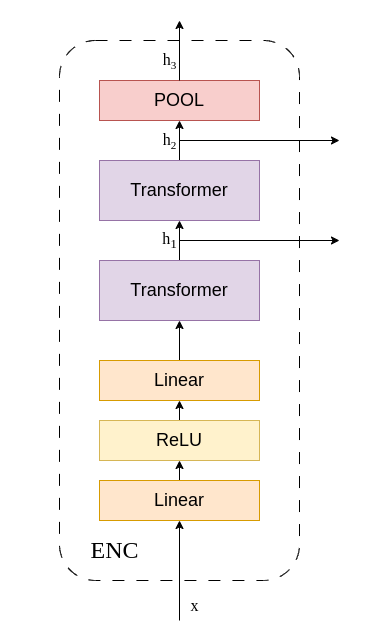
\includegraphics{enc.png}}
        \caption{Baseline Encoder}
        \label{fig:enc}
    \end{subfigure}
    \hfill
    \begin{subfigure}{0.33\textwidth}
        \centering
        \adjustbox{height=5cm,keepaspectratio}{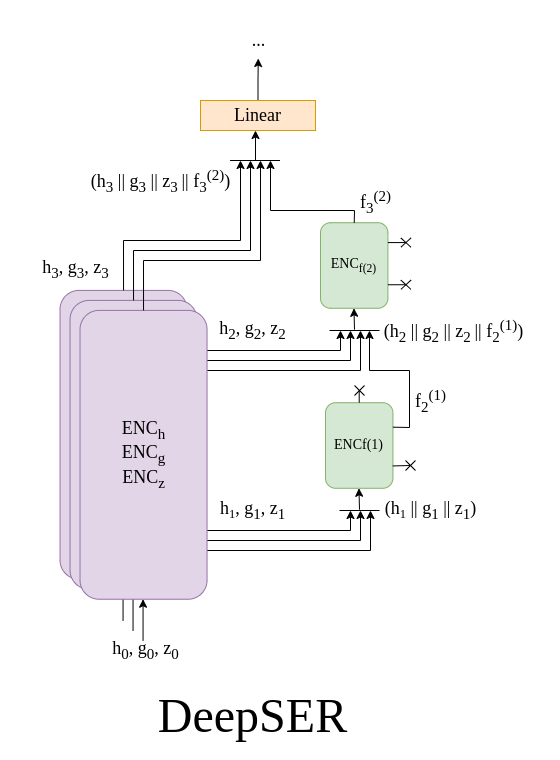
\includegraphics{deep-ser.png}}
        \caption{Baseline DeepSER architecture}
        \label{fig:deepser}
    \end{subfigure}
    \hfill
    % \begin{subfigure}{0.33\textwidth}
    %     \centering
    %     \adjustbox{height=5cm,keepaspectratio}{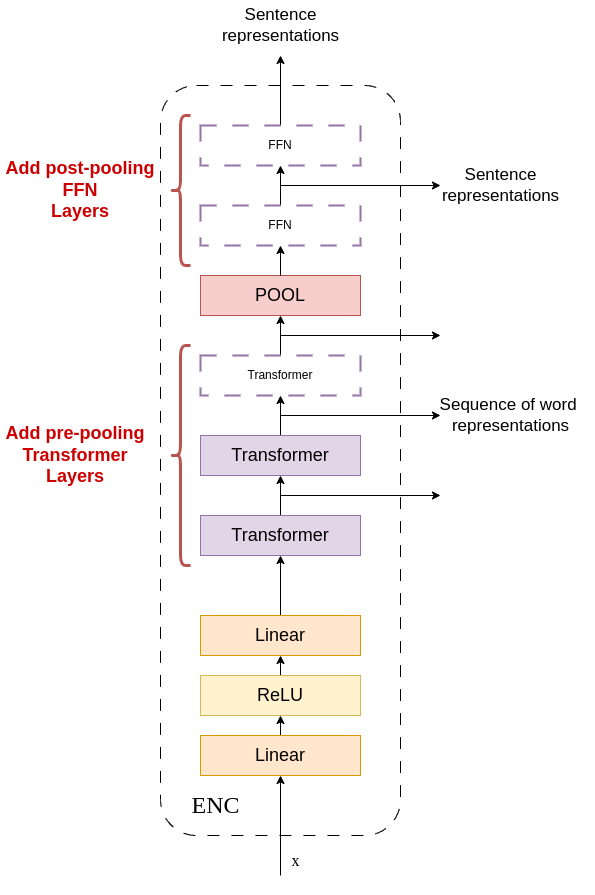
\includegraphics{enc-vardepth.png}}
    %     \caption{VarDepth Encoder}
    %     \label{fig:vardepth}
    % \end{subfigure}
    % \hfill
    \begin{subfigure}{0.33\textwidth}
        \centering
        \adjustbox{height=5cm,keepaspectratio}{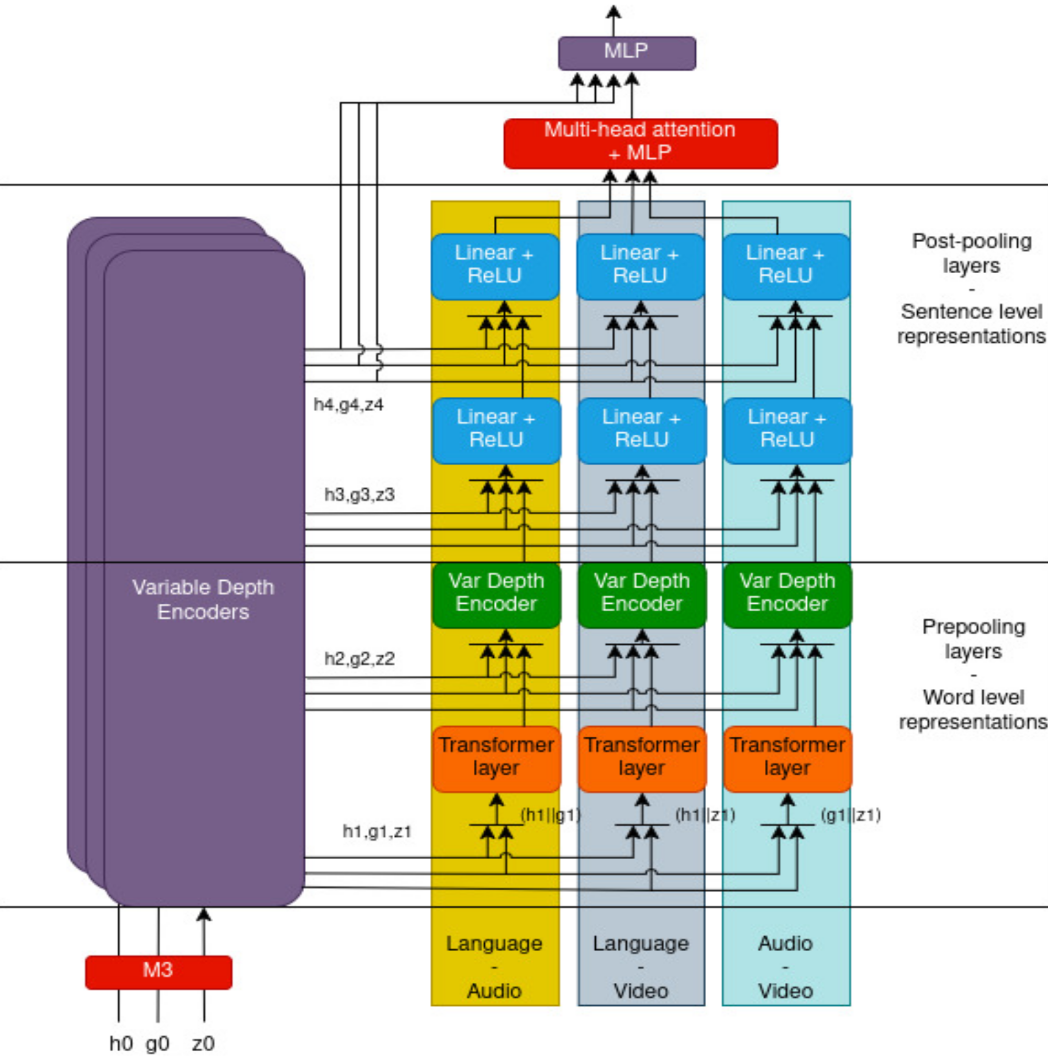
\includegraphics{pairwise.png}}
        \caption{Our proposed Pairwise Fusion architecture (PairwiseVarDepthDeepSER)}
        \label{fig:pairwise}
    \end{subfigure}
    \caption{Architectural components of our multimodal sentiment analysis framework: (a) standard encoder, (b) baseline DeepSER model, (c) our variable-depth encoder modification, and (d) pairwise cross-modal fusion mechanism.}
    \label{fig:architectures}
\end{figure*}

\section{Method}
\subsection{Architecture}
\par At this stage our team experimented with variations of the underlying DeepSER architecture. We designed a generalization of the base encoder that may be initialized with an arbitrary amount of layers. Using this flexible module, we were able to find interesting configurations and architectural improvements. We also conducted experiments with a new DeepSER spin, that performs fusion in a  pairwise fashion. This new model showed significant improvements over the baseline.

\subsubsection{Variable Depth}
\par If someone were to add more layers to the base encoder, they could do so at two different stages: before the pooling layer or after it (see Figure \ref{fig:enc}). The former case is rather simple: simply add more Transformer layers. In the latter case however, there would be no meaning in doing so. After the pooling we no longer have a sequence of words, but a single sentence representation. Hence, the well known self-attention mechanism \cite{attention} loses its intuitive meaning. So, we were led to experiment with our own custom Feed-Forward (FF) layers.
\par To keep computation demands low, we performed such experiments with one Transformer layer before the pooling operation and three FF layers after the pooling (1-3 configuration)\footnote{From now on, we denote by an X–Y configuration the use of an encoder with X pre-pooling layers and Y post-pooling layers}. We yielded the best results by using a special type of Convolutional layers, which apply kernels of size 3, 5 and 7 in parallel and reshape the resultwith a Linear+ReLU. We called the resulting encoder VarDepth and the model utilizing this encoder VarDepthDeepSER. 

\subsubsection{Attention Pooling}
\par We also conducted experiments with an alternative pooling layer. We replaced the original mean-pooling with an attention-based pooling layer. Experiments on a simple 1-0 configuration showed promising results. However, when scaling up, this accuracy gain would gradually vanish.

\subsubsection{Pairwise Fusion}
\par To better capture modality interactions, we replace the single 3‑way VarDepth flow with three separate pairwise VarDepth flows (see Figure \ref{fig:pairwise}). By isolating each pair, we force the network to learn those specific cross‑modal correlations directly, before attempting any higher‑order integration. Similar ideas have been used in \cite{m3} and in \cite{mulT}. Also in \cite{m3} the M3 layer is proposed as a regularization technique. This layer applies masking in some modalities during training, so we will use it in order to avoid overfitting. 
\par In the simplest instantiation, each unimodal leg produces a hierarchy of representations through 2 pre‑pooling Transformer layers followed by a pooling, then 2 post‑pooling layers that refine the fused features. With the same logic more complex models can be created by adding more pre-pooling and more post-pooling fusion layers, using also the appropriate VarDepth unimodal encoders in order to extract all the required hidden representations.  
\par The fusion logic is similar to the DeepSER base model using 2 modalities in each flow instead of 3. In all the pre-pooling layers (except for the last one), the fusion is done with concatenation and a simple 1-layer transformer. In the last pre-pooling layer we use a VarDepth Encoder 3-1. We use this encoder (that applies pooling)  instead of a simple transformer because we need to produce sentence level fused representations, in order to use them in the next layer. If we want to use more layers, we add more transformer layers. Similarly in all the post-pooling layers the fusion is done with concatenation and MLP+ReLU. We can add more of these layers to make the model even deeper.
\par Once each of the three flows yields its final vector, we stack them into a 3‑token sequence and apply a multi‑head self‑attention block. The attention weights reveal which modality‑pair interactions the model deems most informative for a given example. We then mean‑pool across the three tokens, project with a simple MLP, and merge with the unimodal “last‑layer” outputs exactly as in the original DeepSERBase. Finally, we use a linear layer to produce the final decision.
\par This same pattern applies to any choice of pre‑ and post‑pooling layers. In our experiments, we found that the best architecture is the one that uses 4 pre‑pooling and 4 post‑pooling layers.

\subsection{Training Strategy}
\par As far as training is concerned, we first pretrain each modality-specific encoder using self-supervised or supervised objectives (with either freezing or fine-tuning) and then apply ensemble methods—meta-regressor stacking and Model Soup weight averaging \cite{modelsoup} to merge multiple models’ predictions into a more robust final output.

\subsubsection{Encoders Pretraining}
\par To exploit unlabeled data and improve the encoders' generalization capabilities, we designed self-supervised tasks tailored to each modality:
\par{\textbf{Text:}} For the text modality, we treat each token embedding sequence as a denoising autoencoder. During pre-training, we randomly mask 15\% of the tokens and add Gaussian noise to every embedding. The corrupted sequence is fed through the text encoder, and a linear “reconstruction head” maps the final pooled representation back to the average of the original, uncorrupted token embeddings. We minimize mean-squared error (MSE) between the reconstructed and true pooled embeddings. 
\par{\textbf{Audio:}} Audio pre-training follows a SimCLR-style contrastive paradigm. From each raw audio feature sequence, we generate two augmented views by injecting Gaussian noise and applying time-masking to 20\% of the frames. We compute the normalized cosine-similarity matrix between all view pairs, and apply an InfoNCE loss, treating matching views as positives. By pulling together representations of the same clip under different corruptions, the encoder learns invariances critical for downstream emotion recognition.
\par{\textbf{Vision:}} On the visual modality, we mask out 15\% of all frames in each sequence. We compute the target as the per-sample mean of the original features at those masked positions, and feed the corrupted sequence through the VarDepth vision encoder. A three-layer MLP head reconstructs the missing content. We again minimize MSE between reconstruction and target. By integrating context from the remaining frames, the encoder learns motion-sensitive embeddings.
\par Apart from self-supervision, we also pre-trained each modality-specific encoder on the MOSEI sentiment regression task using only the corresponding modality. This setup provides a supervised signal aligned with our final objective. 
\par Each encoder was trained individually, and the best-performing checkpoint (lowest validation loss) was saved.
\par We explored two strategies for incorporating pretrained encoders into our full multimodal models (BaseEnc and PairwiseVarDepthDeepSER):
\begin{itemize}
    \item Frozen Initialization: Pretrained encoder weights were loaded and then frozen during multimodal training.
    \item Trainable Initialization: Pretrained weights were used to initialize the encoders, but all parameters remained trainable during downstream training. This allows the model to adapt to cross-modal interactions.
\end{itemize}


\subsubsection{Meta-Classifier and Model Soup}
\par We first collected predictions from multiple base multimodal models, trained with different seeds and hyperparameters. These included models based on our PairwiseVarDepthDeepSER architecture with various prepool/postpool combinations (e.g., 4-4 and 2-3) and different regularization setups (e.g., mixup, dropout). For each example in the test set, we extracted a vector of regression outputs—one from each base model.
\par These stacked outputs served as input features to a lightweight Linear Meta-Classifier trained to map ensemble predictions to the final target sentiment score. The training was done using mean-squared error (MSE) loss, with a simple fully connected layer acting as the meta-model.
\par We trained the meta-classifier using multiple random seeds and conducted evaluations on a held-out portion (20\%) of the test data to avoid overfitting. 


\section{Setup}
\subsection{Dataset}
\par All experiments are conducted on the CMU-MOSEI dataset, a large-scale multimodal corpus for sentiment and emotion analysis. MOSEI contains over 23,000 video clips from YouTube, each annotated with sentiment scores ranging from –3 (strongly negative) to +3 (strongly positive).

\subsection{Features}
\par We extract three types of modality-specific features for each utterance:
\begin{itemize}
    \item Textual features: 768-dimensional BERT embeddings from the pretrained bert-base-uncased model, obtained by averaging the last four hidden layers for each utterance.
    \item Acoustic features: 74-dimensional vectors from COVAREP, including MFCCs, pitch, and glottal parameters.
    \item Visual features: 35-dimensional facial action units and landmark measurements from FACET.
\end{itemize}

\subsection{Evaluation Metrics}
To assess both regression and classification performance, we report:
\begin{itemize}
    \item Mean Absolute Error (MAE): Mean absolute difference between predicted and ground-truth sentiment scores.
    \item Correlation Coefficient (CorrCoef): Linear correlation between predictions and labels.
    \item 5-class and 7-class Accuracy (acc5, acc7): Accuracy after discretizing continuous predictions into 5 or 7 equally spaced bins.
    \item Binary Accuracy (acc): Accuracy when classifying sentiment as negative (score < 0) vs. non-negative (score ≥ 0).
    \item F1 Score (f1): Harmonic mean of precision and recall for the binary task.
\end{itemize}

\subsection{Experimental Approach}
\par Each configuration is run three times with different random seeds. Reported results are the arithmetic mean over these three runs to account for stochastic variability.

\section{Results}
\subsection{Architectural Experiments}
\par Table \ref{tab:pool} shows the results of the pooling experiments. These experiments took place on a simple VarDepthDeepSER 1-3 model, in order to keep computational demand low and amplify the effects of the pooling layer. For this simple configuration, our attention-based pooling shows constant improvements over the baseline mean pooling. However, when trying to scale up, these improvements gradually vanished. We believe that this is a result of overfitting and may be tackled through more extensive parameter experimentation.
\par Keeping the models simple (not too many total layers), we discovered a very interesting property of the convolutional layers and our attention pooling. Combined, they achieve results similar to the baseline (with notable improvements on Correlation Coefficient and MAE), while using significantly fewer parameters. While not having an exact calculation of the parameter number, we use the average training time per batch on an L4 GPU, as a crude measurement of model complexity. Specifically, the baseline needed approximately 650ms per batch during training. Our approach achieves better results, with only about 250ms per batch. This highlights the promising potential of our proposed improvements.
\par In Table \ref{tab:arch} we compare the DeepSER base model with 3 variations of the Pairwise DeepSER model (2-0, 4-4, 5-5). The (4, 4) model achieves the best results, outperforming the base by approximately 1\% on all metrics. The (2, 2) model yields gains only on acc5, acc7, and MAE, while the (5, 5) model improves all metrics versus DeepSER Base but falls short of the (4, 4) configuration.
\subsection{Training Strategy}
\par We experimented with both the original MEDUSA encoders and our own VarDepth Encoders, used in our best-performing Pairwise DeepSER (prepool=4, postpool=4). Overall, trainable encoders consistently outperformed frozen ones, and fine-tuning directly on the downstream task yielded better results than self-supervised pre-training alone. The results are as shown in Table \ref{tab:training}. 
\par Α particularly striking improvement came from pretraining the Base Encoder on the downstream task, then keeping its weights trainable. This approach not only achieved higher metrics but also proved far more efficient: each modality converged quickly, and the full model stabilized by the third epoch.When training the VarDepth Encoders,  performance gains were marginal or even negligible, suggesting that deeper multimodal fusion layers may overshadow the benefit of unimodal pretraining.
\par While literature supports the importance of modality-specific pretraining, especially in noisy or low-resource modalities, our experiments show limited gains. Possible reasons:
\begin{itemize}
    \item The MOSEI dataset already provides relatively rich multimodal alignment and supervision.
    \item Our fusion architecture is powerful enough to learn useful representations from scratch.
    \item The downstream task may not benefit strongly from unimodal improvements, especially if inter-modal attention compensates for weak encodings.
\end{itemize}
\par We now present the results of our meta-classifier, which was designed to combine and refine predictions from multiple base models.
\par The meta-classifier consistently outperformed individual models across several evaluation metrics, including accuracy, F1 score, correlation coefficient, and mean absolute error (MAE). Notably:
\begin{itemize}
    \item Accuracy and F1 improved across the board.
    \item MAE was consistently reduced, indicating more precise continuous predictions.
    \item Correlation Coefficient increased, suggesting the model better captured the structure of human sentiment ratings.
    \item Slight drops in acc5 and acc7 were observed, likely due to finer-grained error corrections not captured by coarse multiclass thresholds.
\end{itemize}
\par When applying Model Soup, results were further improved or remained on par, with added benefits in stability and robustness across runs. The results are as shown in Table \ref{tab:ensemble}.


\begin{table*}[htbp]
    \centering
    \caption{Comparison between mean pooling and attention pooling}
    \label{tab:pool}
    \begin{tabular}{lcccccc}
    \toprule
    Model & Acc & F1 & Acc5 & Acc7 & Corr & MSE \\
    \midrule
    1-0 mean pooling & 0.830 & 0.830 & 0.528 & 0.516 & 0.727 & 0.576 \\
    1-0 attention pooling & \textbf{0.846} & \textbf{0.848} & \textbf{0.539} & \textbf{0.528} & \textbf{0.742} & \textbf{0.557} \\
     & (+1.6\%) & (+1.8\%) & (+1.1\%) & (+1.2\%) & (+1.5\%) & (-1.9\%) \\
    \bottomrule
    \end{tabular}
\end{table*}
    
\begin{table*}[t]
    \centering
    \caption{Experimental architectures compared with the base model}
    \label{tab:arch}
    \begin{tabular}{lcccccc}
    \toprule
    Model & Acc & F1 & Acc5 & Acc7 & Corr & MAE \\
    \midrule
    DeepSER base & 0.841 & 0.841 & 0.540 & 0.527 & 0.736 & 0.563 \\
    \addlinespace
    VarDepth 1-3 + att pooling & 0.844 & 0.844 & 0.546 & 0.530 & 0.748 & 0.554 \\
     & \footnotesize{(+0.3\%)} & \footnotesize{(+0.3\%)} & \footnotesize{(+0.6\%)} & \footnotesize{(+0.3\%)} & \footnotesize{(+1.2\%)} & \footnotesize{(-0.9\%)} \\
    \addlinespace
    Pairwise DeepSER 2-0 & 0.838 & 0.837 & 0.545 & 0.530 & 0.739 & 0.561 \\
     & \footnotesize{(-0.3\%)} & \footnotesize{(-0.4\%)} & \footnotesize{(+0.5\%)} & \footnotesize{(+0.3\%)} & \footnotesize{(+0.3\%)} & \footnotesize{(-0.2\%)} \\
    \addlinespace
    Pairwise DeepSER 5-5 & 0.848 & 0.850 & 0.544 & 0.529 & 0.741 & 0.554 \\
     & \footnotesize{(+0.7\%)} & \footnotesize{(+0.9\%)} & \footnotesize{(+0.4\%)} & \footnotesize{(+0.2\%)} & \footnotesize{(+0.5\%)} & \footnotesize{(-0.9\%)} \\
    \addlinespace
    Pairwise DeepSER 4-4 & \textbf{0.850} & \textbf{0.851} & \textbf{0.552} & \textbf{0.536} & \textbf{0.745} & \textbf{0.550} \\
     & \footnotesize{(+0.9\%)} & \footnotesize{(+1.0\%)} & \footnotesize{(+1.2\%)} & \footnotesize{(+0.9\%)} & \footnotesize{(+0.9\%)} & \footnotesize{(-1.3\%)} \\
    \bottomrule
    \end{tabular}
\end{table*}

\begin{table*}[t]
    \centering
    \caption{Encoder Training Strategy Comparison}
    \label{tab:training}
    \begin{tabular}{lcccccc}
    \toprule
    \textbf{Model Configuration} & \textbf{Accuracy} & \textbf{F1} & \textbf{acc5} & \textbf{acc7} & \textbf{CorrCoef} & \textbf{MAE} \\
    \midrule
    \multicolumn{7}{l}{\textbf{Base Encoders}} \\
    \cmidrule(lr){1-7}
    Base & 0.8407 & 0.8412 & 0.5397 & 0.5265 & 0.7361 & 0.5630 \\
    SSL + Freeze & 0.8382 & 0.8407 & 0.5402 & 0.5267 & 0.7358 & 0.5660 \\
    SSL + Trainable & 0.8413 & 0.8425 & 0.5446 & 0.5318 & 0.7454 & 0.5537 \\
    Downstream + Freeze & 0.8356 & 0.8345 & 0.5389 & 0.5265 & 0.7207 & 0.5637 \\
    Downstream + Trainable & \textbf{0.8469} & \textbf{0.8486} & 0.5435 & 0.5294 & 0.7418 & 0.5575 \\
    \addlinespace
    \multicolumn{7}{l}{\textbf{VarDepth Encoders}} \\
    \cmidrule(lr){1-7}
    Pairwise 4-4 & \textbf{0.8496} & \textbf{0.8506} & \textbf{0.5520} & \textbf{0.5362} & \textbf{0.7447} & \textbf{0.5495} \\
    SSL + Freeze & 0.8359 & 0.8351 & 0.5262 & 0.5117 & 0.7237 & 0.5918 \\
    SSL + Trainable & 0.8447 & 0.8452 & 0.5437 & 0.5292 & 0.7484 & 0.5549 \\
    Downstream + Freeze & 0.8330 & 0.8347 & 0.5105 & 0.4974 & 0.7124 & 0.6032 \\
    Downstream + Trainable & 0.8422 & 0.8423 & 0.5422 & 0.5265 & 0.7367 & 0.5610 \\
    \bottomrule
    \end{tabular}
\end{table*}

\begin{table*}[t]
    \centering
    \caption{Ensemble Model Performance Comparison}
    \label{tab:ensemble}
    \begin{tabular}{lcccccc}
    \toprule
    \textbf{Model Configuration} & \textbf{Accuracy} & \textbf{F1} & \textbf{Acc5} & \textbf{Acc7} & \textbf{CorrCoef} & \textbf{MAE} \\
    \midrule
    DeepSER Base & 0.832 & 0.832 & 0.534 & 0.521 & 0.728 & 0.570 \\
    \addlinespace
    \multicolumn{7}{l}{\textbf{DeepSER Base Ensemble (hidden dim = 512, batch size = 96)}} \\
    \cmidrule(lr){1-7}
    DeepSER Base (7 models) & 0.839 & 0.839 & 0.524 & 0.510 & 0.751 & 0.574 \\
    Difference from DeepSER & \scriptsize{+0.7\%} & \scriptsize{+0.7\%} & \scriptsize{-1.0\%} & \scriptsize{-1.1\%} & \scriptsize{+2.3\%} & \scriptsize{+0.4\%} \\
    \addlinespace
    \multicolumn{7}{l}{\textbf{PairwiseVarDepth Ensemble with 4 pre- and 4 post-pooling layers}} \\
    \cmidrule(lr){1-7}
    Pairwise 4-4 (9 models) & 0.858 & 0.859 & 0.534 & 0.519 & 0.784 & 0.548 \\
    Difference from Pairwise DeepSER & \scriptsize{+0.8\%} & \scriptsize{+0.8\%} & \scriptsize{-1.8\%} & \scriptsize{-1.7\%} & \scriptsize{+3.9\%} & \scriptsize{-0.2\%} \\
    \addlinespace
    \multicolumn{7}{l}{\textbf{PairwiseVarDepth ensemble with varying numbers of pre- and post-pooling layers}} \\
    \cmidrule(lr){1-7}
    PairwiseVarDepth (11 models) & \textbf{0.863} & \textbf{0.863} & 0.529 & 0.514 & \textbf{0.787} & \textbf{0.539} \\
    Difference from Pairwise DeepSER & \scriptsize{+1.3\%} & \scriptsize{+1.2\%} & \scriptsize{-2.3\%} & \scriptsize{-2.2\%} & \scriptsize{+4.2\%} & \scriptsize{-1.1\%} \\
    \bottomrule
    \end{tabular}
\end{table*}

\section{Conclusions \& Future Work}
\par In this work, we presented a comprehensive exploration of architectural and training improvements for multimodal sentiment analysis, building upon the DeepSER framework. Our primary contribution is the Pairwise VarDepth DeepSER architecture, which explicitly models modality-pair interactions through dedicated fusion flows before performing full integration. This novel approach delivered leading five- and seven-class accuracy with competitive binary results, achieving consistent ~1\% gains in all metrics over the baseline DeepSER across all evaluation metrics. 
\par Our best configuration (4 pre-pooling, 4 post-pooling layers) demonstrated the effectiveness of explicit pairwise modeling in capturing cross-modal dependencies. We also introduced variable-depth encoders with convolutional layers and attention-based pooling mechanisms, which remarkably cut training time by over 60\% without sacrificing performance, highlighting promising computational efficiency gains. 
\par Additionally, our investigation into encoder pre-training strategies revealed that supervised pretraining on the downstream task with trainable weights provided substantial improvements for simpler architectures, though these gains diminished with more complex fusion layers. Our meta-classifier ensemble approach combined with model soup weight averaging consistently enhanced robustness and achieved our strongest results, delivering 86.3\% accuracy, matching state-of-the-art performance on the CMU-MOSEI dataset, while securing the top binary classification scores. 
\par Future work will target systematic hyperparameter searches to fully unlock the potential of our architectural innovations. Additionally, exploring non-linear meta-regressors and uncertainty-aware ensembling could further improve ensemble robustness, while extending pairwise fusion with additional layers and improved regularization may provide a promising direction for advancing multimodal sentiment analysis beyond current capabilities.

\printbibliography

\end{multicols}

\end{document}
